\documentclass[12pt]{article}
\usepackage{graphicx}
\usepackage[margin=0.8in]{geometry}
\begin{document}
{\bf Names:} Jack Bracewell, Milan Misak, Craig Ellis \\
{\bf Usernames:} jb2910, mm5510, ce710 \\
{\bf Group Number: 28}  \\ \\

\section*{Assignment 3: Artificial Neural Network}

\subsubsection*{Discuss how you obtained the optimal topology and optimal values of network parameters. Describe the performance measure you used (and explain why you preferred it over other measures) and the different topologies/parameters you experimented with.}

We read the matlab guide for neural networks, and it suggested that trainrp (Resilient backpropogation) and trainscg (Scaled conjugate gradient propogation) worked well with pattern recognition, a couple of tests using these proved that they performed better than the other functions, but there was not much difference between them. We decided to use trainrp because it appeared to be slightly faster. It was not feasible to test all the combinations of transfer functions with all node layouts so we took the reccomendation of the matlab guide and used tansig on all layers, as suggested for pattern recognition problems. To find the best layout of nodes for each network, we used a brute force search on all combinations of nodes from 1-2 hidden layers and 3:20 nodes per layer. A few manual tests suggested that the optimum layouts would lie within this range, and it took too long to search another dimension.\\
The performance measure we used was training each layout 5 times, and using the average best validation score. We chose to measure the best validation performance opposed to the score when training stopped, in the hope that this best score could be achieved later with measures to avoid overfitting. We repeated this 5 times in order to see how well the layout performed with different training and validation sets, the divide function used was dividerand.


\subsubsection*{Explain what strategy you employed to ensure good generalisation ability of the networks and overcome the problem of overfitting.}

When training the network we started off with a large value max\_fail and trained the network 10 times, storing the one with the best performing validation. max\_fail was then decremented, and a new network was found from 10 iterations. If the performance of the network with the lower max\_fail is better, then max fail is decremented again and the algorithm continues. Otherwise, the network trained with the higher value is returned. This method aims to find the optimum value of max\_fail to train the network with. When using a max\_fail too high, the network will overfit so it needs to be reduced as much as possible to eradicate overfitting, but still be big enough to get over the local spikes in validation performance. 


\subsubsection*{In Part VIII you used the optimal parameters that you found in part VI to train your networks. However, there is a problem with this approach, the data you used for validation at some point will be used for testing in cross-validation. Can you explain why this a problem? Ideally how should you optimise the parameters in cross-validation?}

The validation data used to find the optimal parameters is essentially part of the training data because it is used to decided when to stop training. When this data is used again for cross validation it is not validating the network because the network was designed to be optimal for said data. Ideally, there would be 2 different sets of data used to design the network topology, then to cross validate. Or at least, the data used for validation in designing the topology should be marked in a way so it cannot be used as part of the validation set in cross validation.

\subsubsection*{Is there any difference in the classification performance of the two different classification approaches. Discuss the advantages/disadvantages of using 6 single-output NNs vs. 1 six-output NN.}

Yes, there is a difference in classification performance - the six single-output networks perform very slightly better then the single six-output network. Both the advantages listed below, and the data given later on, show that the six-output network has an average of 1 or 2 percent lower recall and precision rates than the six single-output networks. \\


\begin{itemize}
  \item The advantages of a six-output neural network are: the network will be weighted to give preference to one emotion over another, based on an attribute. For example, an attribute could indicate either emotion 1 or emotion 2 - separately, this gives us little information, but when evaluating both in the same network, perhaps the attribute is more likely to signify emotion 1 over emotion 2. It also takes longer to train, and more space to store,  6 single-output networks than one six-output network.
  \item The advantages of six single-output neural networks are: the networks are likely to be more TODO: accurate, since each one will weight its output focused purely on one emotion. This means weights, etc, will be specific to each tree, and should therefore reduce the number of false positives - the actual emotion is likely to have a higher output than the false positive, and overrule it (TODO: multi-output network is bad because).
\end{itemize}


\subsection*{Implementation details}
\begin{itemize}
  \item Cross-validation is done in much the same way as it was done for Decision Trees, with the exception that we needed two separate functions - one for the six one-output networks, and one for the six-output network. The cross-validation functions are passed the clean data received directly from ANNdata(), which is then split up in to training and validation data on each fold.
  \begin{itemize}
    \item For the six-output network, a network is created and trained using the optimal parameters we found, then used to predict the emotions of the validation inputs. These predictions are then compared to the correct outputs, and used to create the confusion matrix and calculate classification rate. After all the folds an average confusion matrix is constructed and other rates and measures ($F_1$, precision, recall) are calculated.
    \item The six one-output networks were similarly cross-validated, being represented by a cell-array of networks, which were easier to work with. The testANN() function, used to make the predictions, was modified to recognise whether or not the input was a cell-array, and to modify it accordingly, to make predictions (see below).
  \end{itemize}
  \item The outputs of the six one-output networks were combined in the testANN() function, into a single matrix like the one returned by the six-output network. this allowed the same function to be used for predictions (ie. the max value found for each column).
  \item The process of figuring out optimal parameters of networks was made simpler by programatically testing different combinations of numbers of hidden layer nodes. Other parameters such as the number of hidden layers (2) were chosen by trial and error where we tried to minimise the mean square error of validation.
\end{itemize}


\subsection*{Evaluation results}

\subsubsection*{6 1-output networks}

\begin{table}
\centering
\begin{tabular}{r r | r r r r r r}
\multicolumn{8}{c}{Predicted class} \\
&  & Anger & Disgust & Fear & Happiness & Sadness & Surprise \\
\hline
 & Anger            & 10.1 & 0.9  & 0.6 & 0.2  & 1.3 & 0.1  \\
 & Disgust          & 1.7  & 16.2 & 0.1 & 0.6  & 1.1 & 0.1  \\
Actual class & Fear & 0.3  & 0.2  & 9.4 & 0.3  & 0.5 & 1.2  \\
 & Happiness        & 0.1  & 0.6  & 0   & 20.5 & 0.2 & 0.2  \\
 & Sadness          & 1.1  & 2.0  & 0.7 & 0.5  & 8.5 & 0.4  \\
 & Surprise         & 0.2  & 0.1  & 0.9 & 0.3  & 0.3 & 18.9 \\
\end{tabular}
\caption{Confusion matrix}
\end{table}

\begin{table}
\centering
\begin{tabular}{l | r r}
Emotion & Recall rate (\%) & Precision rate (\%) \\
\hline
Anger     & 76.5152 & 74.8148 \\
Disgust   & 81.8182 & 81.0000 \\
Fear      & 78.9916 & 80.3419 \\
Happiness & 94.9074 & 91.5179 \\
Sadness   & 64.3939 & 71.4286 \\
Surprise  & 91.3043 & 90.4306 \\
\end{tabular}
\caption{Recall and precision rates}
\end{table}

\begin{table}
\centering
\begin{tabular}{l | r}
Emotion & \( F_1 \) measure \\
\hline
Anger     & 75.6554 \\
Disgust   & 81.4070 \\
Fear      & 79.6610 \\
Happiness & 93.1818 \\
Sadness   & 67.7291 \\
Surprise  & 90.8654 \\
\end{tabular}
\caption{F1 measures}
\end{table}

Average classification rate = 0.8328 \\ \\
Confusion matrix: the confusion matrix suggests that our neural networks work well. Anger, disgust and sadness are sometimes classified incorrectly as some other emotion from this group. Otherwise the predicted emotions work very well and some misclassifications do not occur at all (or haven't occurred during our testing). For example surprise has never been classified as anger. Classification rate: this is very high as it normally reaches over 80 per cent whenever we run the program. It is a lot higher that last time when we were using decision trees. It also means that our classified is very precise and reliable. Precision/Recall rate TODO

Something like:
Confusion matrix: The happiness tree was very good, perhaps overfit. Disgust and Happiness were quite often misclassified as well as correctly. They probably produced better trees because there was more data for them. Classification rate: The average classification rate is semi-successful as it succeeds most of the time. But it is far from perfect. Precision/Recall rate: The standout results are that sadness and fear are very difficult to identify correctly, most of the time they are not recognised. Wheras Hapiness was easy to recall but also registering many false positives. The anger tree was very cautious in making classifications but when it did, it was very successful.  F-measure: The F measures suggest as suspected that the Disgust and Happiness have well trained trees. Perhaps Sadness and Surprise did not have enough data. Anger is likely an easy emotion to classify given the trees high performance given a relatively small amount of data \\ \\

Confusion matrix: The happiness tree was very good, perhaps overfit. Disgust and Happiness were quite often misclassified as well as correctly. They probably produced better trees because there was more data for them. Classification rate: The average classification rate is semi-successful as it succeeds most of the time. But it is far from perfect. Precision/Recall rate:  F-measure: The F measures suggest as suspected that the Disgust and Happiness have well trained trees. Perhaps Sadness and Surprise did not have enough data. Anger is likely an easy emotion to classify given the trees high performance given a relatively small amount of data \\ \\


\subsubsection*{6-output network}

\begin{table}
\centering
\begin{tabular}{r r | r r r r r r}
\multicolumn{8}{c}{Predicted class} \\
&  & Anger & Disgust & Fear & Happiness & Sadness & Surprise \\
\hline
 & Anger            & 9.1 & 1.8  & 0.4 & 0.4  & 1.4 & 0.1  \\
 & Disgust          & 1.4 & 15.5 & 0.5 & 0.8  & 1.5 & 0.1  \\
Actual class & Fear & 0.4 & 0.3  & 9.3 & 0.1  & 0.6 & 1.2  \\
 & Happiness        & 0.2 & 0.8  & 0   & 20.0 & 0.3 & 0.3  \\
 & Sadness          & 1.2 & 2.2  & 0.5 & 0.6  & 8.5 & 0.2  \\
 & Surprise         & 0   & 0.2  & 1.2 & 0.6  & 0.4 & 18.3 \\
\end{tabular}
\caption{Confusion matrix}
\end{table}

\begin{table}
\centering
\begin{tabular}{l | r r}
Emotion & Recall rate (\%) & Precision rate (\%) \\
\hline
Anger     & 68.9394 & 73.9837 \\
Disgust   & 78.2828 & 74.5192 \\
Fear      & 78.1513 & 78.1513 \\
Happiness & 92.5926 & 88.8889 \\
Sadness   & 64.3939 & 66.9291 \\
Surprise  & 88.4058 & 90.5941 \\
\end{tabular}
\caption{Recall and precision rates}
\end{table}

\begin{table}
\centering
\begin{tabular}{l | r}
Emotion & \( F_1 \) measure \\
\hline
Anger     & 71.3725 \\
Disgust   & 76.3547 \\
Fear      & 78.1513 \\
Happiness & 90.7029 \\
Sadness   & 65.6371 \\
Surprise  & 89.4866 \\
\end{tabular}
\caption{F1 measures}
\end{table}

Average classification rate = 0.8039 \\ 

TODO: Not Crarig


\subsection*{Average performance per fold}

TODO: Not Crarig

\newpage
\subsection*{Code Flowcharts}

\begin{center}
  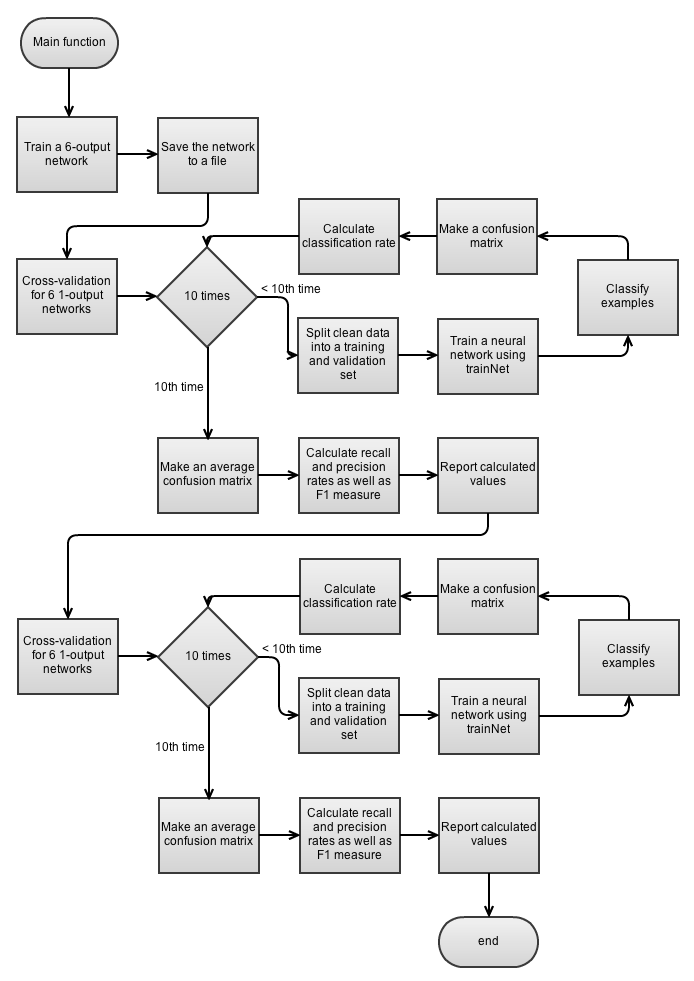
\includegraphics[scale=0.7]{report-images/main.png}
\end{center}

% TODO - trainNet and optimization flowcharts

\end{document}
